\documentclass[useAMS,usenatbib]{mn2e}
\usepackage{natbib}
\usepackage{amssymb}
\usepackage{epsf}
\usepackage{pstricks}
\usepackage{color}
\usepackage{graphicx}
\usepackage{slashed}
\usepackage{relsize}
\usepackage{morefloats}
%\usepackage[font=small,skip=0pt]{caption}
%\usepackage{caption}

%\usepackage {amsmath}
%\usepackage {amsxtra}
%\usepackage {amsbsy}
%\usepackage {amscd}
\usepackage {array}

%\usepackage {graphics}
%\usepackage {amsfonts}
%\usepackage {float}
%\usepackage {indentfirst}
%\usepackage{verbatim}

%\usepackage {a4wide}
%\usepackage {setspace}
%\usepackage{enumitem}

\newcommand{\nat}{Nature}
\newcommand{\mnras}{MNRAS}
\newcommand{\apj}{ApJ}
\newcommand{\apjl}{ApJL}
\newcommand{\apjs}{ApJS}
\newcommand{\aap}{A\&A}
\newcommand{\pasa}{PASA}
\newcommand{\apss}{ApSS}
\newcommand{\araa}{ARAA}
\newcommand{\aj}{Astron. J.}
\newcommand{\aaps}{A\&AS}
\newcommand{\aplett}{Astrophys. Lett.}

\topmargin=-0.4in

%%%%%%%%%%%%%%%%%%%%%%%%%%%%%%%%%%%%%%%%%%%%%%%%%%%%%%%%%%%%%%%%%%%%%%
\bibliographystyle{mn2e}

\begin{document}

\title[A Study of the Multi-frequency Polarization Pulse Profiles of Millisecond Pulsars]{A Study of the Multi-frequency Polarization Pulse Profiles of Millisecond Pulsars}

\author[S. Dai et al.]{S. Dai$^{1,2}$, G. Hobbs$^1$, R. N. Manchester$^1$, W. van Straten$^3$, R. Shannon$^1$, M. Kerr$^1$\\
%\author[S. Dai et al.]{S. Dai$^{1,2}$, G. Hobbs$^2$, R. N. Manchester$^2$, W. van Straten$^3$, R. Shannon$^2$, \\
\newauthor A. Mata$^4$, H. G. Wang$^{5,1}$, C. Tiburzi$^{6,7,1}$, PPTA\\
$^1$CSIRO Astronomy and Space Science, Australia Telescope National Facility, Box 76 Epping NSW 1710, Australia\\
$^2$Department of Astronomy, School of Physics, Peking University, Beijing 100871, China\\
$^3$Centre for Astrophysics and Supercomputing, Swinburne University of Technology, PO Box 218, Hawthorn, VIC 3122, Australia\\
$^4$Center for Advanced Radio Astronomy, University of Texas, Rio Grande Valley,
Brownsville, TX 78520, USA\\
$^5$School of Physics and Electronic Engineering, Guangzhou University, 510006 Guangzhou, China\\
$^6$INAF–Osservatorio Astronomico di Cagliari, Via della Scienza, I-09047 Selargius (CA), Italy\\
$^7$Dipartimento di Fisica, Universit\`a di Cagliari, Cittadella Universitaria, I-09042 Monserrato (CA), Italy\\
}

\maketitle

\begin{abstract}

We present high signal-to-noise ratio, multi-frequency polarization profiles 
for $24$ millisecond pulsars that are being observed as part of the Parkes 
Pulsar Timing Array (PPTA) project. 
%
The pulsars are observed in three bands, centering at $\sim730$, $\sim1400$
and $\sim3100$ MHz, using a dual-band $10\rm{cm}$/$50\rm{cm}$ receiver and the 
central beam of the $20\rm{cm}$ multibeam receiver. 
%
Data sets that have been carefully calibrated over several years are utilized, 
which allows us to study the components and evolution of profiles with 
frequency, and to show previously undetected profile features. 
%
With the high S/N pulse profiles, we show that the overall width of pulse 
profiles at $\sim1400$ MHz is wider than previously thought, with $17$ of the 
$24$ pulsars show emission over more than half of the pulse period. 
%
Both the pulse profile and the position angle variation show complex structures 
and clear evolution with frequency. 
%
However, the frequency evolution of pulse width is weak, and the frequency 
evolution of polarization parameters are different from pulsars to pulsars.
%
%These results support theories that suggest millisecond pulsar emission 
%regions are wider, at least in terms of pulse longitude, than those of the 
%normal pulsars. 
%The magnetic field of millisecond pulsars could be much more complicated 
%than a dipolar structure.
%
%Polarization variations across the profiles are complex, and the observed 
%position angle variations are generally not in accord with the rotating vector 
%model for pulsar polarization. Nevertheless, the polarization properties are 
%broadly similar to those of normal (non-millisecond) pulsars, suggesting that 
%the basic radio emission mechanism is the same in both classes of pulsar.
%The results support the idea that radio emission from millisecond pulsars 
%originates high in the pulsar magnetosphere, probably close to the emission 
%regions for high-energy X-ray and gamma-ray emission. Rotation measures were 
%obtained for all 20 pulsars, eight of which had no previously published 
%measurements.


\end{abstract}



\begin{keywords}
%
pulsars: general
%
\end{keywords}


\section{Introduction}

Millisecond pulsars (MSPs) are a special subgroup of radio pulsars. 
%
Compared with ``normal'' pulsars, they have much shorter spin periods 
and smaller spin-down rates, and therefore have larger characteristic 
ages and weaker implied dipole magnetic fields.
%
The short spin periods and highly stable average pulse shapes of MSPs 
make them powerful tools to investigate various astrophysical phenomena 
using high precision timing of the pulse arrival times~\citep[e.g.,][]{Manchester08}.
%

The Parkes Pulsar Timing Array (PPTA) project (Manchester et al. 2013) 
regularly observes $24$ MSPs. The main goal of the project is to identify 
slight variations in the pulse arrival times from these MSPs that can be 
identified as being caused by gravitational waves passing through the solar 
system.  
%
The search for gravitational waves has been described in other papers (recent 
work includes~\citet{Shannon13b}, Wang et al., Zhu et al.). 
%
To detect gravitational waves, we could observe a larger set of pulsars 
and increase the span of the observations, but also to increase the timing 
precision of the PPTA data set.
%
%requires that the pulse arrival times are measured with 
%a precision and accuracy of $\sim100$ ns over decades. 
%
%This requires that the pulse profiles are measured with high signal-to-noise 
%ratio and are stable over long time spans.  
%
Determining how to improve the timing precision and how much we can improve 
it relies on our understanding of the stability of pulse profiles~\citep[e.g.,][]{Shannon14} 
and also the frequency evolution and polarization properties.
%
For our work we study the large number of well calibrated, high signal-to-noise 
ratio (S/N) multi-frequency polarization profiles that have been obtained as 
part of the PPTA project. 
%

An earlier analysis of the pulse profiles from the PPTA sample was published by
~\citet{Yan11}. This earlier work is extended in this paper as:
%
(1) we include an extra four pulsars that have been recently added to the PPTA sample;
(2) we use more modern pulsar backend instrumentation than was available to~\citet{Yan11};
(3) we use longer data sets enabling higher S/N ratio profiles;
(4) we provide polarization pulse profiles in three independent bands 
(at $10$, $20$ and $50$ cm).~\citet{Yan11} only analysed observations in the $20$ cm band.
%- we compare different models for different pulsar rotation measures
%
We note that we have mainly the same sample of pulsars as was described by \citet{Yan11}, 
but our data sets are independent (i.e., no data is in common between this and the earlier 
publication).

It has been shown that, compared with normal pulsars, the pulse profiles of MSPs are 
much more complicated and cover a much larger fraction of the pulse period~\citep{Yan11}, 
and the PAs are more complex and do not fit the `rotating vector model'~\citep[RVM,][]{Radhakrishnan69}.
%
However, the spectra of MSPs and normal pulsars are similar~\citep{Toscano98,Kramer98,Kramer99}, 
and both of them have features such as high degrees of linear polarization and orthogonal 
mode position angles (PA) jumps~\citep[see e.g.,][]{Thorsett90,Navarro97,Stairs99,Manchester04,Ord04}.
%
To explain the complex pulse profiles, multiple emission cones were proposed 
and discussed by several authors~\citep{Rankin93,Kramer94,Gupta03}. An alternative 
model suggests that the emission beam of a pulsar is filled with randomly 
distributed emission patches~\citep{Lyne88,Manchester95_2,Han01}. The patchy 
model may explain more complicated multi-component and asymmetric pulse profiles.
%

To date, no simple model exists yet that can describe the observations.  
%
This paper is the first in a series of papers that we hope will shed new light on 
the MSP emission mechanism. This first paper is purposely an observationally-based 
publication.  
%
We present the new profiles in the various observing bands and describe how they were 
created. We determine various observationally-derived properties of the profiles (such as 
spectral indices, polarisation fractions, etc.) and study how such parameters vary 
between pulsars and also for different components for a given pulsar.   
%
The data described here will be used in a subsequent paper to study the stability 
of the pulse profiles as a function of time. This sample of pulsars has been chosen for 
high-precision pulsar timing experiments. In a further paper, we will therefore also test 
out new methods~\citep[e.g.,][]{Pennucci14,Liu14} to improve our timing precision using 
frequency-dependent pulse templates.  
%
Our data sets are publically available enabling anyone to compare the actual 
observations with their models of the pulse profiles.
%Although previous studies suggest that MSPs and normal pulsars have 
%similar radiation mechanisms, their emission and polarization properties 
%could be very different.
%%
%The study of polarization pulse profile of MSPs is then not only important 
%for understanding the pulse emission mechanism, the beaming of pulsar 
%radiation and the geometry of the system, but also crucial for the 
%high precision pulsar timing using MSPs, which relys on the highly stable 
%average profiles.
%

%To extend previous studies, the most promising approach is detailed investigations 
%on high signal-to-noise ratio (S/N), multi-frequency polarization profiles of MSPs. 
%%
%High S/N reveals fine structures and low-level emissions of the pulse profile, and
%more polarization features, which improve our understanding of the beaming of radiation
%and emission mechanisem.
%%
%What is more, together with multi-frequency observations, the frequency evolution 
%of both pulse profile and polarization can be investigated.
%
%\citet{Yan11} presented high S/N polarization profiles for $20$ MSPs 
%observed by PPTA project, but only with observations at a central frequency 
%of $1369$ MHz. 
%
%In this paper, we present high S/N, multi-frequency polarization 
%profiles of MSPs, using long PPTA data sets that have been well calibrated.
%%
%We also present new measurements of flux densities and spectral indice, 
%and polarization parameters.
%We are able to split the bands into sub-frequency channels to 
%show the details and evolutions of pulse profile within the bands.
%%
%To investigate pulse profile evolution, we measure the phase position, 
%width and amplitude of different profile components for each sub-frequency 
%channel, and then study their evolution. The spectral indices of different 
%components are also measured.
%%
%The stability of pulse profiles on hour duration are investigated by 
%calculating the shape parameters and studying the morphological variability.
%

Details of the observation, data processing and data access are given in 
Section $2$. Multi-frequency polarization profiles of each MSPs are presented 
in Section $3$.
%
In Section $4$, we present results of flux densities and spectral indices.
%
In Section $5$, the polarization parameters at different frequencies are 
shown.
%
The implications of the results are discussed in Section $6$.


% Explain Yan’s work and why we’re now writing another paper
% We probably should add in loads about Kramer et al., Ord et al. etc. at the start here. I haven’t done that.

	% Explain all the other cool things that we do (or are going to do)


\section{Observations and Analysis}

\subsection{Observations}

We selected observations from the PPTA project, which includes observations 
of $24$ MSPs. 
%
The pulsars are observed regularly, with an approximate observing cadence of 
three weeks, in three bands centred close to $730$, $1400$ and $3100$ MHz, 
using a dual-band $10\rm{cm}$/$50\rm{cm}$ receiver and the central beam 
of the $20\rm{cm}$ multibeam receiver. In each of the bands, the observing 
bandwidth was $64$, $256$ and $1024$ MHz, respectively. 
%
We used both digital polyphase filterbank spectrometers (PDFB4 at $10\rm{cm}$ 
and PDFB3 at $20\rm{cm}$) and coherent dedispersion machines (CASPSR at $50\rm{cm}$). 
%
In Table \ref{obs}, we summarize the observational parameters for the $24$ PPTA MSPs. 
%Other basic pulsar parameters can be obtained from the ATNF 
%Pulsar Catalogue~\citep{Manchester05}.
%
For each band of the MSPs, we present the number of frequency channels across 
the band, the number of bins across the pulse period, the total number 
of observations we used and the total integration time.
%
%
\begin{table*}
\caption{Observational parameters for the $24$ PPTA MSPs.}
\label{obs}
\begin{center}
%\begin{tabular}{lcccccccccccc}
\begin{tabular}{p{1.5cm}p{0.9cm}<{\centering}p{0.9cm}<{\centering}p{0.9cm}<{\centering}p{0.9cm}<{\centering}p{0.9cm}<{\centering}p{0.9cm}<{\centering}p{0.9cm}<{\centering}p{0.9cm}<{\centering}p{0.9cm}<{\centering}p{0.9cm}<{\centering}p{0.9cm}<{\centering}p{0.9cm}<{\centering}}
\hline
PSR         &     \multicolumn{3}{c}{No. of channels}   &   \multicolumn{3}{c}{No. of phase bins}  &    \multicolumn{3}{c}{No. of observation epochs}   &    \multicolumn{3}{c}{Integration time}      \\
%PSR         &         & No. of chan. &          &         & No. of bins &          &         & No. of obs. &          &         & Integ. time &          \\
            &         &                 &          &         &             &          &         &             &          &         &   (h)            &       \\
            & 730 MHz &    1400 MHz     & 3100 MHz & 730 MHz &  1400 MHz   & 3100 MHz & 730 MHz &  1400 MHz   & 3100 MHz & 730 MHz &  1400 MHz        & 3100 MHz    \\
%        & 730 &    1400     & 3100  & 730 &  1400   & 3100 & 730 &  1400  & 3100 & 730 &  1400 & 3100\\
%        &     &    (MHz)    &       &     &  (MHz)  &      &     &  (MHz) &      &     &  (MHz)&     \\
\hline
J0437$-$4715&  256    &    1024         &   1024   &  1024   &  1024       &  2048    &  177    &  669        & 281      &  142.9  &    502.2         &  248.8   \\
J0613$-$0200&  256    &    1024         &   1024   &  1024   &  512        &  512     &  64     &  160        & 111      &  66.0   &    159.3         &  113.9   \\
J0711$-$6830&  256    &    1024         &   1024   &  1024   &  1024       &  1024    &  72     &  161        & 102      &  65.9   &    161.1         &  102.2   \\
J1017$-$7156&  256    &    2048         &   2048   &  1024   &  256        &  512     &  85     &  135        & 73       &  86.5   &    130.4         &  76.3    \\
J1022$+$1001&  256    &    1024         &   1024   &  1024   &  2048       &  2048    &  65     &  148        & 117      &  58.4   &    138.3         &  110.5    \\
						&         &                 &          &         &             &          &         &             &          &         &                  &           \\
J1024$-$0719&  256    &    1024         &   1024   &  1024   &  1024       &  1024    &  34     &  112        & 59       &  36.1   &    111.0         &  61.5     \\
J1045$-$4509&  256    &    2048         &   1024   &  1024   &  512        &  1024    &  63     &  137        & 103      &  42.7   &    138.9         &  104.5    \\ 
J1446$-$4701&  256    &    512          &   1024   &  1024   &  512        &  1024    &  19     &  50         & 9        &  15.2   &    39.4          &  8.8    \\ 
J1545$-$4550&  256    &    1024         &   1024   &  1024   &  512        &  1024    &  15     &  21         & 15       &  13.2   &    20.6          &  12.2   \\ 
J1600$-$3053&  256    &    1024         &   1024   &  1024   &  512        &  512     &  53     &  139        & 106      &  56.6   &    129.9         &  108.0   \\ 
						&         &                 &          &         &             &          &         &             &          &         &                  &          \\
J1603$-$7202&  256    &    2048         &   1024   &  1024   &  1024       &  1024    &  52     &  131        & 49       &  44.4   &    127.4         &  50.6    \\ 
J1643$-$1224&  256    &    2048         &   1024   &  1024   &  512        &  1024    &  53     &  116        & 93       &  53.7   &    117.0         &  93.4     \\ 
J1713$+$0747&  256    &    1024         &   1024   &  1024   &  1024       &  1024    &  66     &  155        & 110      &  67.8   &    132.0         &  107.9    \\ 
J1730$-$2304&  256    &    1024         &   1024   &  1024   &  1024       &  2048    &  57     &  104        & 62       &  51.0   &    105.8         &  62.2    \\ 
%J1732$-$5049&               &                      \\ 
%            &  2048   &     512              37     &  35.8       \\
%            &  1024   &     1024             16     &  14.9       \\
%
%            & &           &                  \\
J1744$-$1134&  256    &    512          &   1024   &  1024   &  1024       &  1024    &  65     &  129        & 96       &  66.0   &    126.7         &  99.5    \\ 
						&         &                 &          &         &             &          &         &             &          &         &                  &          \\
J1824$-$2453&  256    &    2048         &   1024   &  1024   &  256        &  512     &  33     &  88         & 54       &  33.0   &    82.9          &  53.6    \\ 
J1832$-$0836&  256    &    1024         &   1024   &  1024   &  512        &  1024    &  12     &  19         & 11       &  9.0    &    16.9          &  10.1    \\ 
J1857$+$0943&  256    &    1024         &   1024   &  1024   &  1024       &  1024    &  54     &  99         & 68       &  27.8   &    50.9          &  35.5   \\ 
J1909$-$3744&  256    &    1024         &   1024   &  1024   &  512        &  1024    &  95     &  218        & 138      &  91.3   &    191.1         &  129.4   \\ 
J1939$+$2134&  256    &    1024         &   1024   &  512    &  256        &  256     &  58     &  102        & 91       &  26.4   &    49.4          &  46.0    \\ 
						&         &                 &          &         &             &          &         &             &          &         &                  &     \\
J2124$-$3358&  256    &    1024         &   1024   &  1024   &  1024       &  1024    &  40     &  134        & 78       &  20.3   &    68.5          &  40.5    \\ 
J2129$-$5721&  256    &    1024         &   1024   &  1024   &  512        &  512     &  59     &  116        & 17       &  31.1   &    112.6         &  9.0     \\ 
J2145$-$0750&  256    &    1024         &   1024   &  1024   &  2048       &  2048    &  70     &  134        & 117      &  65.1   &    129.3         &  111.2   \\ 
J2241$-$5236&  256    &    1024         &   1024   &  1024   &  512        &  1024    &  75     &  188        & 93       &  69.8   &    152.3         &  92.9   \\ 
\hline
\end{tabular}
\end{center}
\end{table*}


To calibrate the gain and phase of the receiver system, a linearly polarized 
broad-band and pulsed calibration signal is injected to the two orthogonal 
linearly polarized probes through a calibration probe at $45^{\circ}$ to the 
signal probes. The pulsed calibration signal was recorded for $2$ min prior to 
each pulsar observation.
%
Signal amplitudes were placed on a flux density scale using observations of 
Hydra A.
%
All data were recorded using the PSRFITS data format~\citep{Hotan04} with 
$1$-min subintegrations and the full spectral resolution.
%
(for futher details see~\citet{Manchester13}, and references therein). 
%

%Most of the pulsars in the sample show large flux variability at the PPTA 
%observing frequencies due to diffractive and refractive scintillation. 
%We find that for some of the pulsars in the PPTA sample show measured intensities 
%$> 20$ times of the mean; for these observations, Parkes observations can have S/N 
%in excess of larger aperture telescopes such as the Green Bank Telescope and 
%represent average observation with the MeerKAT telescope.
%


\subsection{Analysis}

The data were processed using the PSRCHIVE software package (Hotan et al. 2004). 
To excise radio-frequency interference, we median-filtered each sub-integration 
and removed $5$ per cent of each edge of the bandpass.
%
The polarization was then calibrated by correcting for differential gain and 
phase between the receptors using associated calibration files.
%
For $20\rm{cm}$ observations with the Multibeam receiver, we corrected for 
cross coupling between the feeds through a model derived from observations of 
PSR J0437$-$4715 that covered a wide range of parallactic angles.
%

The Stokes parameters were in accordance with the astronomical conventions described 
by~\citet{vanStraten10}. Stokes $V$ is defined as $I_{\rm{LH}}-I_{\rm{RH}}$, 
using the IEEE definition for sense of circular polarization. 
%
Stokes $L$ was calculated as $L=(Q^2+U^2)^{1/2}$, and the noise bias in $L$ 
was corrected according to~\citet{Lorimer05}, and the similar bias in 
$V$ was corrected as described in~\citet{Yan11}.
%
PAs were calculated as $\psi=0.5\tan^{-1}(U/Q)$, which are absolute 
and measured from celestial north towards east, i.e. counterclockwise on the sky.
%
The error of PA was estimated according to~\citet{Everett01}, and 
the PA curve is plotted only when the linear polarization is greater than 
$4\ \sigma$.
%
The baseline region was computed for all four Stokes-parameter profiles, separately, 
and baselines for each of the Stokes parameter profiles were set to zero mean.
%

In order to add the data in time to form a final mean profile, pulse times of arrival 
were obtained for each observation using an analytic template based on an existing 
high S/N pulse profile. The TEMPO2 pulsar timing package~\citep{Hobbs06}  
was then used to fit pulsar spin, astrometric and binary parameters, and also fit 
harmonic waves if necessary to give ‘white’ timing residuals for each pulsar. Finally, 
the separate observations were summed using this timing model to determine relative 
phases and form the final Stokes-parameter profiles. To give the best possible S/N 
in the final profile, the individual observation profiles were weighted by their
$(\rm{S/N})^2$ when forming the sum profile. 

To form mean polarization profiles, the Faraday rotation across the band should be 
corrected. 
%
According to~\citet{Yan11b}, the interstellar rotation measure (RM) of PPTA MSPs are 
stable, and we used interstellar RM values from~\citet{Yan11}.
%
To account for the contribution of the Earth's ionosphere, we used two ionospheric 
models, the International Reference Ionosphere (IRI) model suggested in Yan et al. 2011b 
and the IonFR model used by~\citet{Sotomayor13}. 
%
We found that the ionospheric RM value from the above two models for a particular 
observation of one pulsar could be significantly different at some epochs. By 
comparing PAs between $50\rm{cm}$ observations at different epochs corrected using 
these two models, we found that the IRI model was more self-consistent. 
%
This might be due to the insufficient coverage of the Global Positioning System (GPS) in 
the southern hemisphere, based on which the IonFR model works.
%
Therefore, we calculated and corrected the ionospheric RM contributions using IRI models 
through our analysis.
%

In Table \ref{psr}, we present basic pulsar parameters for the $24$ MSPs
from the ATNF Pulsar Catalogue~\citep{Manchester05}.
%
For each observing band, we also present the dispersion smearing and the pulse 
broadening time due to scattering (in units of profile bins).
%
The dispersion smearing across each frequency channel is calculated according to, 
%
\begin{equation}
\Delta t_{\rm{DM}}\approx 8.30 \times 10^{6}\ \rm{DM}\ \Delta f\ f^{-3}\ \rm{ms},
\end{equation}
%
where $\Delta f$ is the channel width in MHz, $f$ is the band centre frequency in MHz, 
and the DM is in units of $\rm{cm^{-3}\ pc}$.
%
The pulse broadening time caused by scattering is estimated using the empirical fit 
from \citet{Bhat04}, 
%
\[
\log \tau_{\rm{d}} = -6.46+0.154\log\rm{DM}+1.07(\log\rm{DM})^2
%\log \tau_{\rm{d}} = -6.46+0.154\log\rm{DM}+1.07(\log\rm{DM})^2-(3.86\pm0.16)\log\nu,
\]
%
\begin{equation}
	\qquad\quad\ \ -(3.86\pm0.16)\log(\frac{f}{1000})\ \rm{ms}.
\end{equation}
%

\subsection{Data access}

The raw data and calibration files used in this paper are available from the 
Parkes data archive~\citep[][data.csiro.au]{Hobbs11}.  
%
The scripts used to create the results given in this paper and the resulting averaged 
profiles are available for public access from XXX ({\bf Note to referee: we intend 
to make these data available from the data archive - however, once published we cannot 
change the files and therefore we’ll only make them available when the paper is accepted 
for publication.}). 

\begin{table*}
\caption{Pulsar parameters for the $24$ PPTA MSPs.}
\label{psr}
\begin{center}
\begin{tabular}{lcccccccc}
\hline
PSR         &   P     &       DM          &          &  DM smear &             &          &   $\tau_{\rm{d}}$ &           \\
            &  (ms)   &  ($\rm{cm^{-3}\ pc}$)  &          &   (bin)   &             &          &     (bins)        &           \\
			      &         &                   &  730 MHz & 1400 MHz  & 3100 MHz    & 730 MHz  &     1400 MHz      & 3100 MHz  \\
\hline
J0437$-$4715&         &                   & 7.9      & 0.4       & 0.3         &  0.0     &  0.0              &  0.0     \\
J0613$-$0200&         &                   & 218.0    & 5.2       & 1.8         &  0.3     &  0.02             &  0.0      \\
J0711$-$6830&         &                   & 57.7     & 2.8       & 1.0         &  0.02    &  0.0              &  0.0     \\
J1017$-$7156&         &                   & 693.4    & 4.2       & 2.9         &  15.4    &  0.3              &  0.03    \\
J1022$+$1001&         &                   & 10.7     & 1.0       & 0.4         &  0.0     &  0.0              &  0.0      \\
            &         &                   &          &           &             &          &                   &           \\
J1024$-$0719&         &                   & 21.6     & 1.0       & 0.4         &  0.0     &  0.0              &  0.0      \\
J1045$-$4509&         &                   & 133.9    & 1.6       & 2.2         &  0.6     &  0.03             &  0.0      \\ 
J1446$-$4701&         &                   & 437.8    & 21.1      & 7.3         &  1.9     &  0.08             &  0.01     \\ 
J1545$-$4550&         &                   & 329.2    & 7.9       & 5.5         &  2.6     &  0.1              &  0.01      \\ 
J1600$-$3053&         &                   & 250.3    & 6.0       & 2.1         &  0.9     &  0.04             &  0.0      \\ 
            &         &                   &          &           &             &          &                   &           \\
J1603$-$7202&         &                   & 44.1     & 1.1       & 0.7         &  0.07    &  0.01             &  0.0      \\ 
J1643$-$1224&         &                   & 232.4    & 2.8       & 3.9         &  1.4     &  0.06             &  0.01      \\ 
J1713$+$0747&         &                   & 60.2     & 2.9       & 1.0         &  0.01    &  0.0              &  0.0      \\ 
J1730$-$2304&         &                   & 20.4     & 1.0       & 0.7         &  0.0     &  0.0              &  0.0      \\ 
%
%J1732$-$5049&        &                   &           &           
%            &        &                   &  2.2      &  0.04        \\
%            &        &                   &  3.1      &  0.0         \\
%
%            &        &                   &  &       &            
J1744$-$1134&         &                   & 13.3     & 1.3       & 0.2         &  0.0     &  0.0              &  0.0      \\ 
            &         &                   &          &           &             &          &                   &           \\
J1824$-$2453&         &                   & 675.5    & 4.1       & 5.6         &  34.8    &  0.8              &  0.06     \\ 
J1832$-$0836&         &                   & 178.3    & 4.3       & 3.0         &  0.1     &  0.01             &  0.0      \\ 
J1857$+$0943&         &                   & 42.7     & 2.1       & 0.7         &  0.01    &  0.0              &  0.0      \\ 
J1909$-$3744&         &                   & 60.7     & 1.5       & 1.0         &  0.01    &  0.0              &  0.0      \\ 
J1939$+$2134&         &                   & 392.3    & 9.4       & 3.3         &  3.5     &  0.2              &  0.01     \\ 
            &         &                   &          &           &             &          &                   &           \\
J2124$-$3358&         &                   & 16.0     & 0.8       & 0.3         &  0.0     &  0.0              &  0.0   \\ 
J2129$-$5721&         &                   & 147.1    & 3.5       & 1.2         &  0.1     &  0.01             &  0.0   \\ 
J2145$-$0750&         &                   & 9.7      & 0.9       & 0.3         &  0.0     &  0.0              &  0.0   \\ 
J2241$-$5236&         &                   & 89.8     & 2.1       & 1.5         &  0.01    &  0.0              &  0.0  \\ 
%
\hline
\end{tabular}
\end{center}
\end{table*}
	

%\begin{table*}
%\caption{Observational parameters for the $24$ PPTA MSPs.}
%\begin{center}
%\begin{tabular}{lcccccccc}
%\hline
%PSR         &  Frequency  &  Band width  &  No. of channels & No. of bins & DM smear & $\tau_{\rm{d}}$ & No. of obs. & Integration time \\
%            &  (MHz)      &   (MHz)      &                  &             & (bins)   &   (bins)        &                      &         (h) \\
%\hline
%J0437$-$4715&  730        &   64         &   256    &  1024  &  7.9    &  0.0             &  177   &  142.9    \\
%            &  1400       &   256        &   1024   &  1024  &  0.4    &  0.0             &  669   &  502.2    \\
%            &  3100       &   1024       &   1024   &  2048  &  0.3    &  0.0             &  281   &  248.8    \\
%%
%J0613$-$0200&  730        &   64         &   256    &  1024  &  218.0  &  0.3             &  64    &  66.0     \\
%            &  1400       &   256        &   1024   &  512   &  5.2    &  0.02            &  160   &  159.3    \\
%            &  3100       &   1024       &   1024   &  512   &  1.8    &  0.0             &  111   &  113.9    \\
%%
%J0711$-$6830&  730        &   64         &   256    &  1024  &  57.7   &  0.02            &  72    &  65.9    \\
%            &  1400       &   256        &   1024   &  1024  &  2.8    &  0.0             &  161   &  161.1    \\
%            &  3100       &   1024       &   1024   &  1024  &  1.0    &  0.0             &  102   &  102.2    \\
%%
%J1017$-$7156&  730        &   64         &   256    &  1024  &  693.4  &  15.4            &  85    &  86.5    \\
%            &  1400       &   256        &   2048   &  256   &  4.2    &  0.3             &  135   &  130.4    \\
%            &  3100       &   1024       &   2048   &  512   &  2.9    &  0.03            &  73    &  76.3     \\
%%
%J1022$+$1001&  730        &   64         &   256    &  1024  &  10.7   &  0.0             &  65    &  58.4     \\
%            &  1400       &   256        &   1024   &  2048  &  1.0    &  0.0             &  148   &  138.3    \\
%            &  3100       &   1024       &   1024   &  2048  &  0.4    &  0.0             &  117   &  110.5    \\
%%
%%            &         &          &          &        &          &     &         &     &      \\
%J1024$-$0719&  730        &   64         &   256    &  1024  &  21.6   &  0.0             &  34    &  36.1     \\
%            &  1400       &   256        &   1024   &  1024  &  1.0    &  0.0             &  112   &  111.0    \\
%            &  3100       &   1024       &   1024   &  1024  &  0.4    &  0.0             &  59    &  61.5    \\
%%
%J1045$-$4509&  730        &   64         &   256    &  1024  &  133.9  &  0.6             &  63    &  42.7     \\ 
%            &  1400       &   256        &   2048   &  512   &  1.6    &  0.03            &  137   &  138.9    \\
%            &  3100       &   1024       &   1024   &  1024  &  2.2    &  0.0             &  103   &  104.5    \\
%%
%J1446$-$4701&  730        &   64         &   256    &  1024  &  437.8  &  1.9             &  19    &  15.2     \\ 
%            &  1400       &   256        &   512    &  512   &  21.1   &  0.08            &  50    &  39.4    \\
%            &  3100       &   1024       &   1024   &  1024  &  7.3    &  0.01            &  9     &  8.8      \\
%%
%J1545$-$4550&  730        &   64         &   256    &  1024  &  329.2  &  2.6             &  15    &  13.2     \\ 
%            &  1400       &   256        &   1024   &  512   &  7.9    &  0.1             &  21    &  20.6    \\
%            &  3100       &   1024       &   1024   &  1024  &  5.5    &  0.01            &  15    &  12.2     \\
%%
%J1600$-$3053&  730        &   64         &   256    &  1024  &  250.3  &  0.9             &  53    &  56.6     \\ 
%            &  1400       &   256        &   1024   &  512   &  6.0    &  0.04            &  139   &  129.9    \\
%            &  3100       &   1024       &   1024   &  512   &  2.1    &  0.0             &  106   &  108.0     \\
%%
%%            &         &          &          &        &          &     &         &     &      \\
%J1603$-$7202&  730        &   64         &   256    &  1024  &  44.1   &  0.07            &  52    &  44.4     \\ 
%            &  1400       &   256        &   2048   &  1024  &  1.1    &  0.01            &  131   &  127.4    \\
%            &  3100       &   1024       &   1024   &  1024  &  0.7    &  0.0             &  49    &  50.6     \\
%%
%J1643$-$1224&  730        &   64         &   256    &  1024  &  232.4  &  1.4             &  53    &  53.7     \\ 
%            &  1400       &   256        &   2048   &  512   &  2.8    &  0.06            &  116   &  117.0    \\
%            &  3100       &   1024       &   1024   &  1024  &  3.9    &  0.01            &  93    &  93.4     \\
%%
%J1713$+$0747&  730        &   64         &   256    &  1024  &  60.2   &  0.01            &  66    &  67.8     \\ 
%            &  1400       &   256        &   1024   &  1024  &  2.9    &  0.0             &  155   &  132.0    \\
%            &  3100       &   1024       &   1024   &  1024  &  1.0    &  0.0             &  110   &  107.9    \\
%%
%J1730$-$2304&  730        &   64         &   256    &  1024  &  20.4   &  0.0             &  57    &  51.0     \\ 
%            &  1400       &   256        &   1024   &  1024  &  1.0    &  0.0             &  104   &  105.8    \\
%            &  3100       &   1024       &   1024   &  2048  &  0.7    &  0.0             &  62    &  62.2     \\
%%
%%J1732$-$5049&  730        &            &          &    &               &         &        &       \\ 
%%            &  1400       &   256        &   2048   &  512   &  2.2    &  0.04            &  37    &  35.8     \\
%%            &  3100       &   1024       &   1024   &  1024  &  3.1    &  0.0             &  16    &  14.9     \\
%%
%%            &         &          &          &        &          &     &         &     &      \\
%J1744$-$1134&  730        &   64         &   256    &  1024  &  13.3   &  0.0             &  65    &  66.0     \\ 
%            &  1400       &   256        &   512    &  1024  &  1.3    &  0.0             &  129   &  126.7     \\
%            &  3100       &   1024       &   1024   &  1024  &  0.2    &  0.0             &  96    &  99.5      \\
%%
%J1824$-$2453&  730        &   64         &   256    &  1024  &  675.5  &  34.8            &  33    &  33.0     \\ 
%            &  1400       &   256        &   2048   &  256   &  4.1    &  0.8             &  88    &  82.9     \\
%            &  3100       &   1024       &   1024   &  512   &  5.6    &  0.06            &  54    &  53.6      \\
%%
%J1832$-$0836&  730        &   64         &   256    &  1024  &  178.3  &  0.1             &  12    &  9.0     \\ 
%            &  1400       &   256        &   1024   &  512   &  4.3    &  0.01            &  19    &  16.9     \\
%            &  3100       &   1024       &   1024   &  1024  &  3.0    &  0.0             &  11    &  10.1     \\
%%
%J1857$+$0943&  730        &   64         &   256    &  1024  &  42.7   &  0.01            &  54    &  27.8     \\ 
%            &  1400       &   256        &   1024   &  1024  &  2.1    &  0.0             &  99    &  50.9     \\
%            &  3100       &   1024       &   1024   &  1024  &  0.7    &  0.0             &  68    &  35.5     \\
%%
%J1909$-$3744&  730        &   64         &   256    &  1024  &  60.7   &  0.01            &  95    &  91.3     \\ 
%            &  1400       &   256        &   1024   &  512   &  1.5    &  0.0             &  218   &  191.1    \\
%            &  3100       &   1024       &   1024   &  1024  &  1.0    &  0.0             &  138   &  129.4     \\
%%
%%            &         &          &          &        &          &                 &     &      \\
%\hline
%\end{tabular}
%\end{center}
%\end{table*}
%	
%%
%\begin{table*}
%\setcounter{table}{0}
%\caption{Continued.}
%\begin{center}
%\begin{tabular}{lcccccccc}
%\hline
%PSR         &  Frequency  &  Band width  &  No. of channels & No. of bins & DM smear & $\tau_{\rm{d}}$  & No. of obs. & Integration time \\
%            &  (MHz)      &   (MHz)      &                  &             & (bins)   &   (bins)         &          &        (h) \\
%\hline
%J1939$+$2134&  730        &   64         &  256     &  512   &  392.3     &  3.5          &  58    &  26.4     \\ 
%            &  1400       &   256        &  1024    &  256   &  9.4       &  0.2          &  102   &  49.4    \\
%            &  3100       &   1024       &  1024    &  256   &  3.3       &  0.01         &  91    &  46.0     \\
%%
%J2124$-$3358&  730        &   64         &  256     &  1024  &  16.0      &  0.0          &  40    &  20.3     \\ 
%            &  1400       &   256        &  1024    &  1024  &  0.8       &  0.0          &  134   &  68.5    \\
%            &  3100       &   1024       &  1024    &  1024  &  0.3       &  0.0          &  78    &  40.5     \\
%%
%J2129$-$5721&  730        &   64         &  256     &  1024  &  147.1     &  0.1          &  59    &  31.1     \\ 
%            &  1400       &   256        &  1024    &  512   &  3.5       &  0.01         &  116   &  112.6    \\
%            &  3100       &   1024       &  1024    &  512   &  1.2       &  0.0          &  17    &  9.0     \\
%%
%J2145$-$0750&  730        &   64         &  256     &  1024  &  9.7       &  0.0          &  70    &  65.1     \\ 
%            &  1400       &   256        &  1024    &  2048  &  0.9       &  0.0          &  134   &  129.3    \\
%            &  3100       &   1024       &  1024    &  2048  &  0.3       &  0.0          &  117   &  111.2     \\
%%
%J2241$-$5236&  730        &   64         &  256     &  1024  &  89.8      &  0.01         &  75    &  69.8     \\ 
%            &  1400       &   256        &  1024    &  512   &  2.1       &  0.0          &  188   &  152.3    \\
%            &  3100       &   1024       &  1024    &  1024  &  1.5       &  0.0          &  93    &  92.9     \\
%%
%\hline
%\end{tabular}
%\end{center}
%\end{table*}
	


\section{Multi-frequency Polarization Profiles}

In this section, we present the multi-frequency polarization profiles. 
%
PA variations and polarization profiles in all three bands for each MSP 
are shown, with a zoom-in of the baseline presented in the lower part of each 
panel.
%
In Table \ref{tableWidth}, we present the overall pulse width and pulse 
widths at $50$ per cent of the peak flux density (W50) and $10$ per cent 
of the peak (W10), all in degrees of longitude, where $360$ is equivalent 
to the pulse period or $1.0$ in pulse phase, and in milliseconds.
%
The overall pulse width is measured from the first point to the last point 
where the pulse intensity significantly exceeds the baseline 
noise~\citep{Yan11}, with pulse profiles in the $20$ cm band since they 
normally have the highest S/N.
%
%
%The next column gives the minimum number of identifiable
%pulse components in the pulse profile. A component is identified
%by a peak or, for overlapping components a significant inflection,
%in the pulse profile. 
%
In Fig. \ref{w50}, the W10 and W50 are plotted against frequency for each MSP. 
%

Compared with previous studies, we have obstained much higher S/N pulse 
profiles, and have multi-frequency and polarization information at the same 
time.
%
According to Table \ref{tableWidth}, we increase the overall width by $\sim10$ per 
cent on average, compared with ~\citet{Yan11}. 
%
We discover weak components and emissions that unknown before for PSR J2145$-$0750, 
PSR J1603$-$7202 and PSR J2241$-$5236.
%
We also show much more details of the PA curves, including new orthogonal 
transitions for PSR J1643$-$1224, PSR J0711$-$6830, PSR J0437$-$4715, PSR J2124$-$3358, 
PSR J2129$-$5721 and PSR J2241$-$5236; and new non-orthogonal transitions for 
PSR J1045$-$4509, PSR J1857$+$0943 and PSR J2124$-$3358.
%
The frequency evolution of pulse profiles and polarization parameters 
can be clearly seen for all MSPs.

In the following subsections, we present and discuss the multi-frequency 
polarization profile of each MSPs.
%

\begin{table*}
\begin{center}
\caption{Pulse width for PPTA MSPs.}
\label{tableWidth}
\begin{tabular}{lccccccc}
\hline
PSR              &     Overall width     &               &   $W_{10}$       &                  &      &      $W_{50}$       &                      \\
								 &      1400 MHz         &  730 MHz      &          1400 MHz           &    3100 MHz      &  730 MHz      &          1400 MHz           &    3100 MHz       \\
								 &        (deg)          &    (deg)   &         (deg)          &     (deg)   &   (deg)   &         (deg)          &     (deg)  \\
\hline
J0437$-$4715     &  299.5      & 130.5     & 63.4   & 18.6   & 15.4  & 8.9   & 5.6             \\
J0613$-$0200     &  178.2      & 105.9     & 109.1  & 105.4  & 10.5  & 54.9  & 30.4             \\
J0711$-$6830     &  283.3      & 180.9     & 168.2  & 167.8  & 131.4  & 124.3  & 108.7             \\
J1017$-$7156     &  70.6       & 22.2      & 21.7   & 34.4   & 16.1  & 10.7  & 11.0             \\
J1022$+$1001     &  72.1       & 41.9      & 43.0   & 35.8   & 16.5  & 21.1  & 8.2             \\
	               &        &      &   &   &   &   &              \\
J1024$-$0719     &  277.7      & 123.6     & 109.6  & 113.7  & 67.3  & 35.7  & 32.0             \\
J1045$-$4509     &  357.9      & 70.3      & 69.7   & 66.6   & 33.5  & 36.6  & 35.7             \\
J1446$-$4701     &  93.0       &           & 45.2   &        &       & 12.2  &              \\
J1545$-$4550     &  243.8      &           & 56.8   &        &       & 12.8  &              \\
%J1446$-$4701     &  93.0       &           & 45.2   &        & 11.7  & 12.2  & 8.8             \\
%J1545$-$4550     &  243.8      &           & 56.8   & 45.5   &       & 12.8  & 9.2             \\
J1600$-$3053     &  77.5       & 48.6      & 41.3   & 42.1   & 11.2  & 9.3   & 22.7             \\
	               &        &      &   &   &   &   &              \\
J1603$-$7202     &  239.3      & 48.3      & 41.8   & 38.5   & 32.4  & 29.4  & 7.0             \\
J1643$-$1224     &  231.8      & 83.8      & 72.6   & 65.7   & 32.8  & 24.9  & 20.5             \\
J1713$+$0747     &  131.3      & 42.3      & 30.3   & 29.6   & 16.4  & 8.8   & 8.3             \\
J1730$-$2304     &  247.7      & 68.9      & 76.0   & 73.0   & 34.2  & 43.2  & 43.8             \\
J1732$-$5049     &        &      &   &   &   &   &              \\
	               &        &      &   &   &   &   &              \\
J1744$-$1134     &  204.1      & 24.0      & 21.9   & 20.1   & 13.1  & 12.3  & 8.8             \\
J1824$-$2452     &  269.6      & 219.1     & 191.0  & 170.0  & 113.4  &115.4   &7.7              \\
J1832$-$0836     &  285.3      &           & 244.1  &   &       & 113.2  &              \\
%J1832$-$0836     &  285.3      &           & 244.1  & 287.3  &       & 113.2  & 6.3             \\
J1857$+$0943     &  358.3      & 219.0     & 202.4  & 203.4  & 42.4  & 35.2  & 31.2             \\
J1909$-$3744     &  189.5      & 13.1      & 11.0   & 9.2    & 6.9  &  5.3   & 4.3             \\
	               &        &      &   &   &   &   &              \\
J1939$+$2134     &  355.8      & 207.0     & 199.3  & 204.5  & 195.1  &182.1   & 10.5              \\
J2124$-$3358     &  358.9      &           & 269.7  & 282.9  &       & 37.5  & 31.8             \\
J2129$-$5721     &  159.2      & 37.5      & 60.0   & 88.4   & 22.9  & 25.5  & 53.8             \\
J2145$-$0750     &  277.3      & 94.1      & 93.6   & 91.1   & 9.1   & 7.6   & 7.8             \\
J2241$-$5236     &  221.2      & 18.8      & 20.3   & 21.0   & 10.3  & 10.6  & 9.8             \\
\hline
\end{tabular}
\end{center}
\end{table*}

\begin{figure*}
\begin{center}
\includegraphics[width=6 in]{w50.ps}
\caption{Pulse widths at $10$ and $50$ per cent of the peak flux density, 
both in degrees of longitude. Red and blue points represent W10 and W50, respectively.}
\label{w50}
\end{center}
\end{figure*}

\subsection{PSR J0437$-$4715}

The top panel of Fig. \ref{0437} shows the polarization pulse profiles of the 
strongest PPTA MSP, PSR J0437$-$4715.
%
At $1369$ MHz, our results are in good agreement with previously published 
works~\citep{Johnston93,Manchester95_1,Navarro97,Yan11}, which present 
multiple overlapping components and complex polarization variations across 
the pulse profile. 
%
%There are multiple overlapping components, and the present results show that 
%the pulse profile extends over at least 85 per cent of the pulse period. The 
%notches in Stokes I and L discussed by Navarro et al. (1997) and Dyks, Rudak & Rankin
%(2007) are clearly visible in the central expanded plot. The observed PA variations 
%cannot be described by the RVM, even if orthogonal mode jumps are taken into account. 
%There is a clear orthogonal mode transition in both linear and circular polarization 
%very close to the main profile peak and a non-orthogonal PA transition around
%pulse phase −0.23 (Manchester & Johnston 1995; Navarro et al. 1997). We also observe 
%a probable non-orthogonal transition near pulse phase 0.35.
%
The profile of total intensity shows clear frequency development. As the 
frequency decreases, both the leading and trailing emissions becomes stronger.
%
At lower frequencies, the main pulse split into two peaks and the second peak
becomes stronger than the first peak.
%
The PA curves change dramatically in different bands. While the orthogonal 
transition close to the main profile peak exists in all three bands, previously
reported non-orthogonal transitions at $1369$ MHz disappear in other two bands,
and new transitions and discontinuous features can be observed at $728$ MHz 
and $3100$ MHz bands.
%

%Fig. \ref{0437d} shows the mean pulse profile evolution both across and within bands. 
%In the left panel, we can see that from the high frequency to the low frequency,  
%both the leading and trailing emissions grow stronger and results in a wider central 
%peak. 
%%
%At lower frequencies, it is clear that the main peak of the profile has two components, 
%and the second one becomes stronger.
%%
%In the right panel, we show that within each band, the pulse profiles evolve with 
%frequency and results in significant phase shifts. 
%%
%However, such features can be due to both intrinsic pulse profile evolution and 
%inaccurate DM.

\begin{figure*}
\begin{center}
\includegraphics[width=6 in]{0437.ps}
\caption{Multi-frequency polarization profiles for PSR J0437$-$4715. 
The right-side panels present the total intensity $I$ (black, blue and red
line for the $3100$, $1369$ and $728$ MHz band, respectively, as 
indicated), linearly polarized intensity L (magenta line) and circularly 
polarized intensity (cyan line).
%
On the left side of each profile, the PA of the linearly polarized 
emission and the low-level details of the polarization profiles are 
shown.
%
The lower part of the left panel shows the phase-resolved spectral index. 
The red dashed line represents the average spectral index with its uncertainty 
indicated by the yellow region.
%
The lower part of the right panel shows the phase-resolved fractional linear 
polarization, and the black, blue and red points represent the $3100$, $1369$ 
and $728$ MHz band, respectively. 
}
\label{0437}
\end{center}
\end{figure*}

\subsection{PSR J0613$-$0200}

The middle panel of Fig. \ref{0613} shows the polarization pulse profiles of 
PSR J0613$-$0200.
%
At $1369$ MHz, our results are in good agreement with previously published
results~\citep{Ord04,Yan11}. 
%
Our high S/N profiles provide more details in the PA curve, and we show that 
the PA curves are complex and very different in three bands. 
%
At $1369$ MHz, the discontinuous PA at the leading edge of the trailing 
component reported by ~\citet{Yan11} are not observed, and the PA curve seems 
to be continuous.
%
The main pulse of the profile shows clear frequency evolution, and most 
significantly, the trailing peak becomes much stronger at low frequencies 
relative to the rest of the profile and split into two peaks as previously
observed by ~\citet{Stairs99}.
%
From the high frequencies to low frequencies, the fractional linear 
polarization increases, and the trailing component becomes high linear 
polarized. 
%
At $728$ MHz, the circular polarization swaps sign compared to higher 
frequencies.
%
\begin{figure*}
\begin{center}
\includegraphics[width=6 in]{0613.ps}
\caption{Multi-frequency polarization profiles for PSR J0613$-$0200. 
The right-side panels present the total intensity $I$ (black, blue and red
line for the $3100$, $1369$ and $728$ MHz band, respectively, as 
indicated), linearly polarized intensity L (magenta line) and circularly 
polarized intensity (cyan line).
%
On the left side of each profile, the PA of the linearly polarized 
emission and the low-level details of the polarization profiles are 
shown.
%
The lower part of the left panel shows the phase-resolved spectral index. 
The red dashed line represents the average spectral index with its uncertainty 
indicated by the yellow region.
%
The lower part of the right panel shows the phase-resolved fractional linear 
polarization, and the black, blue and red points represent the $3100$, $1369$ 
and $728$ MHz band, respectively. 
}
\label{0613}
\end{center}
\end{figure*}


%The left panel of Fig. \ref{0613d} shows that as frequency decreases, the central component
%of the mean pulse profile dimnishes and the trailing component increases significantly, 
%which agrees with ~\citet{Stairs99}.
%%
%The main central pulse has multiple components which show quite different frequency 
%developments.
%%
%The pulse profile evolution within each band is not obvious from the differences between 
%profiles, but is clear from the phase shifts. 

\subsection{PSR J0711$-$6830}

The bottom panel of Fig. \ref{0711} shows the polarization pulse profiles 
of PSR J0711$-$6830.
%
At $1369$ MHz, our results are in good agreement with previously published
results~\citep{Ord04,Yan11}. 
%
The double-peak weak component following the second peak is clear.
%
The orthogonal mode transition after the peak of the leading component 
is confirmed, and possible orthogonal mode transitions at the trailing edge 
of the main peak are observed at $1369$ MHz and disappear at lower frequencies.
%
Except for that at lower frequencies, the leading component becomes stronger  
relative to the main pulse and the fractional linear polarization of the 
main peak increase significantly, the frequency evolution of the profile 
is not significant.

\begin{figure*}
\begin{center}
\includegraphics[width=6 in]{0711.ps}
\caption{Multi-frequency polarization profiles for PSR J0711$-$6830. 
The right-side panels present the total intensity $I$ (black, blue and red
line for the $3100$, $1369$ and $728$ MHz band, respectively, as 
indicated), linearly polarized intensity L (magenta line) and circularly 
polarized intensity (cyan line).
%
On the left side of each profile, the PA of the linearly polarized 
emission and the low-level details of the polarization profiles are 
shown.
%
The lower part of the left panel shows the phase-resolved spectral index. 
The red dashed line represents the average spectral index with its uncertainty 
indicated by the yellow region.
%
The lower part of the right panel shows the phase-resolved fractional linear 
polarization, and the black, blue and red points represent the $3100$, $1369$ 
and $728$ MHz band, respectively. 
}
\label{0711}
\end{center}
\end{figure*}

%
%Fig. \ref{0711d} shows that the pulse profile frequency development both across and 
%within bands is not significant, although from $10\rm{cm}$ to $20\rm{cm}$ the leading 
%peak grows stronger.  
%

\subsection{PSR J1017$-$7156}

The top panel of Fig. \ref{1017} shows the polarization pulse profiles of 
PSR J1017$-$7156.
%
Our results are in good agreement with and extend previously published 
results~\citep{Keith12}. 
%
We show that the PA variations are more complex than was observed in 
previous work.
%
%At the trailing edge of the main pulse, we observe a probable orthogonal 
%mode transition.
%
Both the linear and circular polarisation shows significant evolution 
with frequency, and the circular polarization close to phase $0$ swaps sign 
at $728$ MHz. 
%
The trailing emission becomes stronger at higher frequencies.

%Fig. \ref{1017d} shows that the mean pulse profile develops with frequency. Even through 
%the S/N of profiles is not very high, we can still see structures in the profile differences 
%and the drifts of phase shift.


\begin{figure*}
\begin{center}
\includegraphics[width=6 in]{1017.ps}
\caption{Multi-frequency polarization profiles for PSR J1017$-$7156. 
See Fig. \ref{0437} for further details.}
\label{1017}
\end{center}
\end{figure*}

\subsection{PSR J1022$+$1001}

The middle panel of Fig. \ref{1022} shows the polarization pulse profiles 
of PSR J1022$+$1001.
%
Our results are in good agreement with previously published results
~\citep{1022Kramer99,Stairs99,Ord04,Yan11}.
%
The PA variation generally fits the RVM in all three bands, but near the 
centre of the profile, it is discontinuous in the $10$cm bands and shows 
glitch in the $20$cm and $50$cm bands as reported by~\citet{Yan11}.
%
The relative strength of the two main peaks evolves dramatically with 
frequency.
%
While the second peak keeps highly linearly polarized, the first peak 
depolarizes rapidly.

\begin{figure*}
\begin{center}
\includegraphics[width=6 in]{1022.ps}
\caption{Multi-frequency polarization profiles for PSR J1022$+$1001. 
See Fig. \ref{0437} for further details.}
\label{1022}
\end{center}
\end{figure*}

%The left panel of Fig. \ref{1022d} shows that across bands, the profile evolves dramatically. 
%While the first peak diminishes, the second peak becomes dominating.
%%
%Even within the bands, the frequency development is clear, especially in the $20$cm 
%band, the relative amplitudes of two peaks change significantly and we can see drifts 
%of phase shift.
%


%
\subsection{PSR J1024$-$0719}

The bottom panel of Fig. \ref{1024} shows the polarization pulse profiles of 
PSR J1024$-$0719.
%
At $1369$ MHz, our results are in good agreement with previously published
results~\citep{Ord04,Yan11}. 
%
Besides the flat PA curve across the main part of the profile as 
previously reported, we also show the PAs of the trailing component which 
varies across the profile.
%
From high frequencies to low frequencies, the leading component and the 
trailing component of the profile become relatively stronger and the peak 
just after the main peak becomes weaker.

\begin{figure*}
\begin{center}
\includegraphics[width=6 in]{1024.ps}
\caption{Multi-frequency polarization profiles for PSR J1024$-$0719. 
See Fig. \ref{0437} for further details.}
\label{1024}
\end{center}
\end{figure*}

%However, at $728$ MHz, as the linear polarization of the trailing component becomes 
%stronger, we observed new features in the PA curve (at phase $0.65$). 

%The left panel of Fig. \ref{1024d} shows that from high frequencies to low 
%frequencies, the leading component and the trailing component become stronger and 
%the peak just after the main peak becomes weaker.
%%
%The profile frequency development within bands is weak as shown from the 
%differences, but in the $20$cm band, the drifts of phase shift is clear.

%
\subsection{PSR J1045$-$4509}

The top panel of Fig. \ref{1045} shows the polarization pulse profiles of 
PSR J1045$-$4509.
%
At $1369$ MHz, our results are in good agreement with previously published
results~\citep{Yan11}, and confirm the leading emission which is joined to 
the main pulse by a low-level bridge of emission.
%
We show the complex PA curve with more details, and determine the PA of the 
low-level bridge connecting the leading emission and the main pulse.
%
At the leading edge of the main pulse, there is a non-orthogonal transition 
rather than a orthogonal transition expected by ~citet{Yan11}.
%
The PA of the low-level bridge emission seems to be discontinuous with 
the rest of the PA variations and could be an orthogonal transition.
%
Except for that at low frequencies, the peak at the trailing edge of the 
main peak disappears and the fractional linear polarization of the trailing 
emission decreases, the profile evolution is not significant.

%The left panel of Fig. \ref{1045d} shows that from high frequencies to low 
%frequencies, the component at the trailing edge of the main pulse gradually 
%diminishes while the component at the leading edge of the main pulse appears 
%in the $20$cm band and disappears again in the $50$cm band.
%%
%The leading emission around phase $-0.5$ becomes stronger from $10$cm to $20$cm, 
%but seems to be weaker at $50$cm.
%%
%The profile frequency development within bands is weak as shown from the 
%differences, but the drifts of phase shift is clear.

\begin{figure*}
\begin{center}
\includegraphics[width=6 in]{1045.ps}
\caption{Multi-frequency polarization profiles for PSR J1045$-$4509. 
See Fig. \ref{0437} for further details.}
\label{1045}
\end{center}
\end{figure*}

\subsection{PSR J1446$-$4701}

The middle panel of Fig. \ref{1446} shows the polarization pulse profiles of 
PSR J1446$-$4701.
%
At $1369$ MHz, our results are generally consistent with previously published
results~\citep{Keith12}.
%
The PAs are flat over the main pulse, but show variations over the leading and 
trailing emissions.
%
%Although the S/N of the profiles in the $10$cm and $50$cm bands are low, we 
%can see the fractional linear polarization increases as the frequency decreases.

\begin{figure*}
\begin{center}
\includegraphics[width=6 in]{1446.ps}
\caption{Multi-frequency polarization profiles for PSR J1446$-$4701. 
See Fig. \ref{0437} for further details.}
\label{1446}
\end{center}
\end{figure*}

\subsection{PSR J1545$-$4550}

The bottom panel of Fig. \ref{1545} shows the polarization pulse profiles of 
PSR J1545$-$4550.
%
At $1369$ MHz, \citet{Burgay13} shows an component around phase $0.35$ that 
we do not see in our analysis. We have confirmed with the HTRU collaboration 
that this extra component was caused by an error in their analysis.  
%
Apart from this, our profiles are consistent in all three frequency bands.
%
We also show that the low-level emissions could extend over at least $80$ 
per cent of the pulse period.

\begin{figure*}
\begin{center}
\includegraphics[width=6 in]{1545.ps}
\caption{Multi-frequency polarization profiles for PSR J1545$-$4550. 
See Fig. \ref{0437} for further details.}
\label{1545}
\end{center}
\end{figure*}

\subsection{PSR J1600$-$3053}

The top panel of Fig. \ref{1600} shows the polarization pulse profiles of 
PSR J1600$-$3053.
%
At $1369$ MHz, our results are generally consistent with previously published
results~\citep{Ord04,Yan11}.
%
The leading component of the main pulse becomes weaker at low frequencies 
relative to the main peak.
%
The central part of the pulse profile depolarizes rapidly as frequency goes 
down. 
%
We see a sign swap of the circular polarization between $3100$ and 
$1369$ MHz, and at $728$ MHz, the circular polarization becomes almost 
$0$ across the whole profile.

%The left panel of Fig. \ref{1600d} shows that from high frequencies to low 
%frequencies, the leading peak of the main pulse becomes weaker. 
%%
%Within in the $20$cm band, we find that the leading component becomes weaker, 
%and the centroid of the profile shifts towards the main peak.  
%high frequencies, but can be clearly seen in the linear polarization, a leading 
%peak, a central part with two components and a trailing peak. 
%
%As frequency decreases, the central part of linear polarization becomes 
%significantly weaker, 
%while the trailing peak grows stronger.
%
%At the same time, the leading part of the total intensity diminishes and its 
%double components becomes clear.
%
%At low frequencies, the circular polarization diminishes, and the PA of the central 
%component of the pulse reverse.
%


\begin{figure*}
\begin{center}
\includegraphics[width=6 in]{1600.ps}
\caption{Multi-frequency polarization profiles for PSR J1600$-$3053. 
See Fig. \ref{0437} for further details.}
\label{1600}
\end{center}
\end{figure*}

\subsection{PSR J1603$-$7202}

The middle panel of Fig. \ref{1603} shows the polarization pulse profiles of 
PSR J1603$-$7202.
%
At $1369$ MHz, our results are in good agreement with previously published
results~\citep{Ord04,Yan11}.
%
The broad low-level feature preceding the main pulse and the double-peak trailing 
pulse can be clearly identified.
%
We find that there are low-level emissions connecting the main pulse and the 
double-peak trailing pulse.
%
The relative strength of the two main peaks evolves significantly with frequency.
%
As frequency goes down, the second main peak becomes highly circular polarized, 
and the low-level emissions almost disappear.

\begin{figure*}
\begin{center}
\includegraphics[width=6 in]{1603.ps}
\caption{Multi-frequency polarization profiles for PSR J1603$-$7202. 
See Fig. \ref{0437} for further details.}
\label{1603}
\end{center}
\end{figure*}

%The left panel of Fig. \ref{1603d} shows that from high frequencies to low 
%frequencies, the main peak of the mean pulse profile becomes much weaker 
%and both the broad low-level leading emission and the double-peak trailing pulse 
%diminish.
%both the total intensity and the circular 
%polarization of the leaing peak become much weaker compared to those of the second 
%peak, but its associated linear polarization grows stronger while the linear 
%polarization of the second peak significantly decreases.
%
%At low frequencies, we can clearly see a bridge of emission connecting the main 
%pulse and the double-peak trailing pulse, but as frequency decreases, both features 
%become much weaker and can be barely seen at $728$ MHz.
%
%The PA curve also show significantly evolution across the bands, especially for the 
%region between two main peaks. 
%
%While the deep reverse peak diminishes at low frequencies, a new bump appears.
%In the right panel, we can see clear profile development within the $20$cm band, 
%which shows that the main peak becomes weaker and the emission between two peaks 
%becomes stronger. 
%%
%The phase shifts also indicate that the centroid of the profile shifts towards 
%second peak.


\subsection{PSR J1643$-$1224}

The bottom panel of Fig. \ref{1643} shows the polarization pulse profiles of 
PSR J1643$-$1224.
%
At $1369$ MHz, our results are in good agreement with and extend previously published
results~\citep{Ord04,Yan11}.
%
The PA of the broad feature preceding the main pulse is determined and 
found to be not only discontinuous with the rest of the PA variation, but 
also show an orthogonal transition.
%
While the linear and circular polarization show clear frequency development,
the total intensity does not evolve with frequency significantly.

\begin{figure*}
\begin{center}
\includegraphics[width=6 in]{1643.ps}
\caption{Multi-frequency polarization profiles for PSR J1643$-$1224. 
See Fig. \ref{0437} for further details.}
\label{1643}
\end{center}
\end{figure*}

%The mean pulse profile evolves little with frequency, except for that the emission 
%at the leading edge of the main pulse disappears at lower frequencies.
%%
%Within each bands, the profile development is not obvious, but we can still see 
%the drifts of phase shift.

\subsection{PSR J1713$+$0747}

The top panel of Fig. \ref{1713} shows the polarization pulse profiles of 
PSR J1713$+$0747. 
%
At $1369$ MHz, our results are consistent with previously published results
~\citep{Ord04,Yan11}, showing the almost complete linear polarized leading and 
trailing components.
%
We detect weak emissions at phase $\sim-0.2$ at $1369$ MHz, and increase the 
overall width from $104^{\circ}$ to $131^{\circ}$. 
%
The non-orthogonal transition preceding the trailing pulse component reported 
by ~citet{Yan11} is observed at $728$ and $3100$ MHz, but not at $1369$ MHz 
where the PA curve is continuous.
%
The linear polarization of the leading and trailing components become stronger 
at low frequencies relative to the rest of the profile.

%The left panel of Fig. \ref{1713d} shows that from high frequencies to low 
%frequencies, we can see that the second component of the profile gradually merges 
%into the main peak.
%%
%The pulse profile evolutions within each bands are significant, and we can see 
%clear drifts of phase shift, which could be due to both profile evolution and 
%DM effects.

\begin{figure*}
\begin{center}
\includegraphics[width=6 in]{1713.ps}
\caption{Multi-frequency polarization profiles for PSR J1713$+$0747. 
See Fig. \ref{0437} for further details.}
\label{1713}
\end{center}
\end{figure*}

\subsection{PSR J1730$-$2304}

The middle panel of Fig. \ref{1730} shows the polarization pulse profiles of 
PSR J1730$-$2304.
%
At $1369$ MHz, our results are consistent with previously published results
~\citep{Ord04,Yan11}. 
%
We clearly show the weak leading and trailing components already reported, 
and detect weaker leading component not discovered before, which increases 
overall width from $232^{\circ}$ to $248^{\circ}$.
%
The pulse profile is very complex, with four clear peaks across the main pulse.
%
The relative strength of these four peaks changes dramatically in different 
bands. While at $3100$ MHz the second peak is the strongest, at $728$ the third 
becomes stronger. 
%
As frequency goes down, the second peak depolarizes rapidly.
%
The PA variations is also complex and are very different in three bands.

\begin{figure*}
\begin{center}
\includegraphics[width=6 in]{1730.ps}
\caption{Multi-frequency polarization profiles for PSR J1730$-$2304. 
See Fig. \ref{0437} for further details.}
\label{1730}
\end{center}
\end{figure*}

%The mean pulse profile of this MSP have multiple peaks, and the left panel of 
%Fig. \ref{1730d} shows that as the frequency decreases, the amplitudes of different 
%peaks evolve dramatically and could either increase or decrease. 
%%
%The pulse profile evolutions within each bands are significant, and we can see 
%clear drifts of phase shift, which could be due to both profile evolution and 
%DM effects.

%\subsection{J1732$-$5049}
%
%Fig. \ref{1732p} shows the polarization pulse profiles of J1732$-$5049. 
%At $1369$ MHz, our results are in good agreement with previously published 
%results~\citep{Yan11}.

%\begin{figure*}
%\begin{center}
%\includegraphics[width=6 in]{1732prof.ps}
%\caption{Total intensity $I$ (thick solid line), linearly polarized intensity L
%(blue thin line) and circularly polarized intensity (red thin line).}
%\label{1732p}
%\end{center}
%\end{figure*}

\subsection{PSR J1744$-$1134}

The bottom panel of Fig. \ref{1744} shows the polarization pulse profiles of 
PSR J1744$-$1134.
%
At $1369$ MHz, our results are consistent with previously published results
~\citep{Yan11}.
%
The multiple-component precursor is clearly identified and no significant 
post-cursor component is observed.
%
While the PAs of the main pulse show smooth decrease, those of the precursor 
have clear structures and do not simply connect with the rest of the PA 
variations.
%
The shape of the PA curves are similar in three bands.
%
The main pulse is highly linearly polarized from $728$ to $3100$ MHz. 
The circular polarizaion of main pulse grows stronger from $3100$ to $1369$ MHz, 
but diminish at $728$ MHz.

\begin{figure*}
\begin{center}
\includegraphics[width=6 in]{1744.ps}
\caption{Multi-frequency polarization profiles for PSR J1744$-$1134. 
See Fig. \ref{0437} for further details.}
\label{1744}
\end{center}
\end{figure*}

%The left panel of Fig. \ref{1744d} shows that the mean pulse profile evolution with 
%frequency is not obvious. For the precursor, it seems that the second peak becomes 
%weaker as frequency decreases.
%%
%However, we can still see significant drifts of phase shifts.


\subsection{PSR J1824$-$2452}

The top panel of Fig. \ref{1824} shows the polarization pulse profiles of 
PSR J1824$-$2452.
%
At $1369$ MHz, our results are consistent with and extend previously published 
results~\citep{Yan11}.
%
The weak component around phase $-0.4$ is clearly shown and is highly 
linearly polarized. 
%
At $1369$ MHz, we also show that there are low-level bridge emissions 
connecting the two the main components of the pulse profile.
%
The PAs of preceding components are continuous themselves, but are 
discontinuous with the rest of the PA variations.
%
The frequency evolution of the total intensity is significant. The first 
main peak observed at $1369$ MHz and the trailing component grow rapidly 
relative to rest of the profile as frequency goes down, while the leading 
component diminish at low frequencies.

%From the left panel of Fig. \ref{1824d}, we see that from high frequencies to 
%low frequencies, the leading peak becomes stronger and stronger, while the main 
%peak becomes weaker.
%%
%At the same time, while the trailing component of the second peak increasing 
%significantly, the leading component of the first peak diminishes.
%%
%The profile evolution within the $20$cm band is obvious as shown in the right 
%panel. It seems that the main peak is shifting which results in the drift 
%of phase shifts.

\begin{figure*}
\begin{center}
\includegraphics[width=6 in]{1824.ps}
\caption{Multi-frequency polarization profiles for PSR J1824$-$2452. 
See Fig. \ref{0437} for further details.}
\label{1824}
\end{center}
\end{figure*}

\subsection{PSR J1832$-$0836}

The middle panel of Fig. \ref{1832} shows the polarization pulse profiles of 
PSR J1832$-$0836.
%
At $1369$ MHz, our results are consistent with and extend previously published 
results~\citep{Burgay13}.
%
The components around phase $-0.45$ and $-0.08$ are highly linearly polarized. 
%
The PAs around phase $-0.05$ and $0.3$ seem to be discontinuous, but is hard 
to confirm due to the low S/N.

\begin{figure*}
\begin{center}
\includegraphics[width=6 in]{1832.ps}
\caption{Multi-frequency polarization profiles for PSR J1832$-$0836. 
See Fig. \ref{0437} for further details.}
\label{1832}
\end{center}
\end{figure*}


\subsection{PSR J1857$+$0943}

The bottom panel of Fig. \ref{1857} shows the polarization pulse profiles of 
PSR J1857$+$0943.
%
At $1369$ MHz, our results are generally consistent with previously published 
results~\citep{Yan11}.
%
We show more details of the PA variation, which is very complex and inconsistent
with the RVM.
%
At leading edge of the main pulse, the PA decreases rapidly followed by an 
orthogonal mode transition. 
%
Around phase $0.05$, there is evidence of a non-orthogonal transition.
%
Close to the peak of the interpulse, the PA shows discontinuity at $1369$ MHz, 
but becomes continuous at $3100$ MHz.
%
Both the main pulse and the interpulse have multiple components and evolve 
with frequency, and at $728$ MHz there is a new linear polarization component 
appearing close to the center of the main pulse.

\begin{figure*}
\begin{center}
\includegraphics[width=6 in]{1857.ps}
\caption{Multi-frequency polarization profiles for PSR J1857$+$0943. 
See Fig. \ref{0437} for further details.}
\label{1857}
\end{center}
\end{figure*}

%The left panel of Fig. \ref{1857d} shows that across the bands, the main pulse 
%shape, which is consist of the main pulse and an interpulse, does not evolve 
%very much.
%%
%However, the components of both the interpulse and the main pulse show 
%variations with frequency. 
%%
%The weak component preceding the main pulse can be identified, and diminishes 
%as frequency increases, which agrees with ~\citet{Thorsett90}.
%%
%The profile evolution with bands and the drifts of phase shift are not obvious. 

\subsection{PSR J1909$-$3744}

The top panel of Fig. \ref{1909} shows the polarization pulse profiles of 
PSR J1909$-$3744.
%
At $1369$ MHz, our results are generally consistent with results of~\citet{Ord04,Yan11}, 
showing a narrow main pulse and a weak feature preceding the main pulse by 
about $0.45$ in phase.
%
The frequency evolution of pulse profile is hard to see, however, the fractional 
linear polarization increases as the frequency decreases.

%The left panel of Fig. \ref{1909d} shows that the mean pulse profile evolution 
%across bands seem to be tiny, only with slightly width increasing.
%%
%But within the $20$cm band, it is clear that the profile shifts and results in 
%the drift of phase shifts, which could be due to DM.

\begin{figure*}
\begin{center}
\includegraphics[width=6 in]{1909.ps}
\caption{Multi-frequency polarization profiles for PSR J1909$-$3744. 
See Fig. \ref{0437} for further details.}
\label{1909}
\end{center}
\end{figure*}

\subsection{PSR J1939$+$2134}

The middle panel of Fig. \ref{1939} shows the polarization pulse profiles of 
PSR J1939$+$2134.
%
At $1369$ MHz, our results are generally consistent with previously published 
results~\citep{Yan11}.
%
As explained in ~\citet{Yan11}, because of the high $DM/P$, our observations 
are significantly affected by DM smearing, and we do not see the secondary 
maxima at the trailing edges of both the main pulses and interpulse
~\citep{Thorsett90,Stairs99,Ord04}.
%
We confirm the existence of weak components preceding both the main pulse 
and interpulse and show that they are highly linear polarized, and therefore 
rule out the possibility of undetected RFI or instrumental problems.
%
Our results show stronger left-circular emission in the main pulse compared 
to ~\citep{Yan11}.
%
The interpulse becomes stronger relative to the main pulse at lower frequencies.
%
The fractional linear polarization of the main pulse increases significantly 
as frequency decreases while that of the interpulse decreases.

\begin{figure*}
\begin{center}
\includegraphics[width=6 in]{1939.ps}
\caption{Multi-frequency polarization profiles for PSR J1939$+$2134. 
See Fig. \ref{0437} for further details.}
\label{1939}
\end{center}
\end{figure*}

%The left panel of Fig. \ref{1939d} shows that from high frequencies to the low 
%frequencies, the interpulse becomes stronger. 
%%
%Within all three bands, both the main pulse and the interpulse show profile 
%development, and the phase shifts significantly drift.


\subsection{PSR J2124$-$3358}

The bottom panel of Fig. \ref{2124} shows the polarization pulse profiles of 
PSR J2124$-$3358.
%
At $1369$ MHz, the complex profile we show here is generally consistent with 
previously published results~\citep{Yan11}.
%
We are able to provide more details of the PA variation and show that it has 
complex structures.
%
At $1369$ MHz, around phase $0.03$ and $-0.5$, there are evidences of two 
orthogonal mode transitions.
%
At $3100$ MHz, around phase $0.1$, there is a non-orthogonal transition of 
$\sim120^{\circ}$.
%
The frequency evolution of pulse profile is relatively weak, but we can 
still see that the trailing edge of the main pulse becomes stronger at 
lower frequencies and the main peak splits into two peaks.
%
The fractional linear polarization of the main pulse increases at lower 
frequencies.

\begin{figure*}
\begin{center}
\includegraphics[width=6 in]{2124.ps}
\caption{Multi-frequency polarization profiles for PSR J2124$-$3358. 
See Fig. \ref{0437} for further details.}
\label{2124}
\end{center}
\end{figure*}

%The left panel of Fig. \ref{2124d} shows that the main pulse of mean  
%profile has multipole components and the component at the trailing edge of 
%the main pulse becomes as strong as the main peak at lower frequencies. 
%%
%The component at phase $-0.4$, which is almost $100\%$ linear polarized, 
%also becomes stronger at low frequencies.
%%
%The pulse profile evolution and phase shifts within bands are not very 
%obvious.

\subsection{PSR J2129$-$5721}

The top panel of Fig. \ref{2129} shows the polarization pulse profiles of 
PSR J2124$-$5721.
%
At $1369$ MHz, our results are in good agreement with and extend previously 
published results~\citep{Yan11}.
%
The weaker leading shelf of emission extends to at least phase of $-0.4$, and 
the post-cursor clearly has multiple components.
%
We show more details of PA in the trailng edge of the main pulse.  
%
The PA decrease across the main pulse, and then increase quickly followed 
by an orthogonal mode transition.
%
From high frequencies to low frequencies, the trailing main-pulse component 
diminishes rapidly, and the second component of the main pulse becomes stronger
than the first component.
%
The fractional linear polarization of the main pulse increases as frequency 
decreases.

%The left panel of Fig. \ref{2129d} shows that from high frequencies to low 
%frequencies, the trailing main-pulse component diminishes, and the second 
%component of the main pulse becomes much stronger.
%%
%We can see slightly profile evolution within bands from the right panel, and 
%the phase shifts drift.

\begin{figure*}
\begin{center}
\includegraphics[width=6 in]{2129.ps}
\caption{Multi-frequency polarization profiles for PSR J2129$-$5721. 
See Fig. \ref{0437} for further details.}
\label{2129}
\end{center}
\end{figure*}

\subsection{PSR J2145$-$0750}

The middle panel of Fig. \ref{2145} shows the polarization pulse profiles of 
PSR J2145$-$0750.
%
At $1369$ MHz, our results are in good agreement with and extend reviously 
published results~\citep{Yan11}.
%
Around phase $0.4$, there are evidences of low-level emissions which 
significantly extends the overall width of this MSPs from $187^{\circ}$ to 
$277^{\circ}$.
%
At $728$ MHz, a new discontinuous feature appears at the trailing edge of 
the main peak. 
%
The trailing emission and the weak leading component become stronger relative 
to the main pulse at lower frequencies, but the PA curves are generally similar 
in three bands.

\begin{figure*}
\begin{center}
\includegraphics[width=6 in]{2145.ps}
\caption{Multi-frequency polarization profiles for PSR J2145$-$0750. 
See Fig. \ref{0437} for further details.}
\label{2145}
\end{center}
\end{figure*}

%The left panel of Fig. \ref{2145d} shows that the most significant pulse 
%profile evolution is that the trailing part of the main pulse and the leading 
%component of the main pulse become stronger.
%%
%Within $10$cm and $20$cm bands, the profile evolution can be seen and the 
%phase shifts drift significantly.

\subsection{PSR J2241$-$5236}

The bottom panel of Fig. \ref{2241} shows the polarization pulse profiles of 
PSR J2241$-$5236.
%
At $1369$ MHz, our results generally agree with and extend reviously published 
results~\citep{Keith11}.
%
We show a new low-level component around phase $0.4$ with a width of $\sim 0.2$.
%
We also show more details of the complex PA variations and there are evidences 
of two orthogonal mode transitions close to the peak.
%
The frequency evolution of pulse profile is hard to see, but the fractional 
linear polarization increases at lower frequencies.

\begin{figure*}
\begin{center}
\includegraphics[width=6 in]{2241.ps}
\caption{Multi-frequency polarization profiles for PSR J2241$-$5236. 
See Fig. \ref{0437} for further details.}
\label{2241}
\end{center}
\end{figure*}

%\begin{figure*}
%\begin{center}
%\includegraphics[width=6 in]{overallWidth.ps}
%\caption{Over all pulse width measured from the first point to the 
%last point where the pulse intensity significantly exceeds the 
%baseline noise (more than $3$ times the baseline rms noise in several 
%adjacent bins)}
%\label{overallWidth}
%\end{center}
%\end{figure*}

%The left panel of Fig. \ref{2241d} shows that the mean pulse profile evolution 
%is not significant. 
%%
%Within the $10$cm band, there are evidences of pulse profile evolution, and the 
%phase shifts show drifts.

\section{Flux Densities and Spectral indices}

In Table \ref{tableFlux}, we present the flux densities and spectral indices 
for all MSPs.
%
Firstly, the mean flux density $S=\langle I\rangle$ of three bands averaged over all 
observations and its uncertainty are given. 
%
Then, the root mean square (rms) fluctuation in individual-observation flux 
densities are presented. Finally, we show the spectral indices.
%
In Fig. \ref{index}, the flux densities are plotted against frequency for each 
MSPs.
%

Compared with ~\citet{Yan11}, the mean flux densities of several MSPs in the $20$ cm 
band show significant differences, which is caused by interstellar scintillation effects.
%
Although we are averaging over a much longer time-span and a larger number of observations, 
we find that measurements of flux densities could still be biased by diffractive 
scintillations and the distributions of flux density are clearly non-gaussian.
%
From Fig. \ref{index}, we can see that a single power-law can fit the spectra 
of most MSPs. Exceptions are PSR J1600$-$3053 and PSR J1713$+$0747, whose spectra show 
flattening at lower frequencies.
%
The spectral indices are consistent with results presented in ~\citet{Toscano98} within 
the measurement uncertainties, but have much smaller uncertainties because of our 
better measurements of flux densities. 
%
However, compared with ~\citet{Kramer99}, the spectral indices show differences 
clearly larger than the uncertainties.
%
Such discrepancies could be due to flux density measurements biased by scintillation 
effects, and also the narrower frequency range we are using.
%
We derive a mean spectral index of $-1.8\pm0.1$, which is consistant with previous 
results and support the idea that MSPs and normal pulsars have similar emission 
characteristics.
%


\begin{table*}
\centering
\caption{Flux densities and spectral indices for PPTA MSPs.}
\label{tableFlux}
\begin{tabular}{lccccccc}
\hline
PSR              &    $S_{730}$   &   $S_{RMS,730}$  &    $S_{1400}$    &   $S_{RMS,1400}$  &    $S_{3100}$    &   $S_{RMS,3100}$  & Spectral index \\
								 &     (mJy)      &      (mJy)       &     (mJy)        &      (mJy)       &      (mJy)       &      (mJy)       &     $\alpha$   \\
\hline
 J0437$-$4715  &  364.3$\pm$ 19.2 &  255.2 &  150.2$\pm$ 1.6  &  42.2 &  35.6$\pm$ 1.2  &  20.5 &  -1.7$\pm$ 0.1    \\
 J0613$-$0200  &  6.7  $\pm$ 0.3  &  2.3   &  2.25 $\pm$ 0.03 &  0.4  &  0.45$\pm$ 0.01 &  0.1  &  -1.90$\pm$ 0.08    \\
 J0711$-$6830  &  11.4 $\pm$ 1.0  &  8.5   &  3.7  $\pm$ 0.4  &  5.7  &  0.72$\pm$ 0.04 &  0.4  &  -1.91$\pm$ 0.07    \\
 J1017$-$7156  &  2.5  $\pm$ 0.1  &  0.8   &  0.99 $\pm$ 0.04 &  0.4  &  0.21$\pm$ 0.01 &  0.1  &  -1.7$\pm$ 0.1    \\
 J1022$+$1001  &  14.2 $\pm$ 2.8  &  22.9  &  4.9  $\pm$ 0.4  &  4.6  &  1.18$\pm$ 0.03 &  0.4  &  -1.73$\pm$ 0.08    \\
               &	                &        &                  &       &                 &       &                 \\
 J1024$-$0719  &  5.6  $\pm$ 0.8  &  4.9   &  2.3  $\pm$ 0.2  &  1.7  &  0.52$\pm$ 0.01 &  0.1  &  -1.7$\pm$ 0.1    \\
 J1045$-$4509  &  9.2  $\pm$ 0.2  &  1.8   &  2.74 $\pm$ 0.04 &  0.5  &  0.48$\pm$ 0.01 &  0.1  &  -2.05$\pm$ 0.06    \\
 J1446$-$4701  &    $\pm$   &     &    $\pm$  &    &   $\pm$  &    &  $\pm$     \\
 J1545$-$4550  &    $\pm$   &     &    $\pm$  &    &   $\pm$  &    &  $\pm$     \\
 J1600$-$3053  &  2.9  $\pm$ 0.1  &  0.4   &  2.44 $\pm$ 0.04 &  0.4  &  0.84$\pm$ 0.02 &  0.2  &  -0.9$\pm$ 0.3    \\
               &	                &        &                  &       &                 &       &                 \\
 J1603$-$7202  &  10.9 $\pm$ 0.7  &  4.9   &  3.5  $\pm$ 0.2  &  1.7  &  0.55$\pm$ 0.06 &  0.4  &  -2.0$\pm$ 0.2    \\
 J1643$-$1224  &  12.4 $\pm$ 0.2  &  1.4   &  4.68 $\pm$ 0.06 &  0.7  &  1.18$\pm$ 0.02 &  0.2  &  -1.63$\pm$ 0.03    \\
 J1713$+$0747  &  10.1 $\pm$ 0.8  &  6.2   &  9.1  $\pm$ 0.7  &  8.4  &  2.6 $\pm$ 0.2  &  1.6  &  -1.0$\pm$ 0.3    \\
 J1730$-$2304  &  11.5 $\pm$ 0.5  &  3.9   &  4.0  $\pm$ 0.2  &  2.0  &  1.7 $\pm$ 0.2  &  1.5  &  -1.5$\pm$ 0.3    \\
 J1732$-$5049  &    $\pm$  &    &   $\pm$  &    &   $\pm$  &    &  $\pm$    \\
               &	                &        &                  &       &                 &       &                 \\
 J1744$-$1134  &  8.0  $\pm$ 0.7  &  5.7   &  3.2  $\pm$ 0.3  &  3.2  &  0.77$\pm$ 0.05 &  0.5  &  -1.63$\pm$ 0.07    \\
 J1824$-$2452  &  11.4 $\pm$ 0.5  &  2.9   &  2.30 $\pm$ 0.05 &  0.4  &  0.39$\pm$ 0.01 &  0.1  &  -2.3$\pm$ 0.2    \\
 J1832$-$0836  &	                &        &                  &       &                 &       &                 \\
 J1857$+$0943  &  10.4 $\pm$ 0.4  &  3.0   &  5.1  $\pm$ 0.3  &  2.9  &  1.2 $\pm$ 0.1  &  0.9  &  -1.4$\pm$ 0.2    \\
 J1909$-$3744  &  4.9  $\pm$ 0.3  &  3.1   &  2.5  $\pm$ 0.2  &  3.2  &  0.76$\pm$ 0.04 &  0.5  &  -1.29$\pm$ 0.07    \\
               &	                &        &                  &       &                 &       &                 \\
 J1939$+$2134  &  67.8 $\pm$ 2.7  &  20.9  &  15.2 $\pm$ 0.6  &  6.2  &  1.82$\pm$ 0.09 &  0.9  &  -2.50$\pm$ 0.06    \\
 J2124$-$3358  &  19.3 $\pm$ 2.7  &  17.2  &  4.5  $\pm$ 0.2  &  2.2  &  0.82$\pm$ 0.01 &  0.1  &  -2.09$\pm$ 0.05    \\
 J2129$-$5721  &  5.9  $\pm$ 0.5  &  3.9   &  1.28 $\pm$ 0.09 &  1.0  &  0.34$\pm$ 0.05 &  0.2  &  -2.1$\pm$ 0.4    \\
 J2145$-$0750  &  27.4 $\pm$ 3.4  &  28.5  &  10.3 $\pm$ 1.0  &  11.2 &  1.75$\pm$ 0.07 &  0.8  &  -2.0$\pm$ 0.1    \\
 J2241$-$5236  &  11.9 $\pm$ 1.8  &  16.2  &  1.95 $\pm$ 0.09 &  1.2  &  0.35$\pm$ 0.01 &  0.1  &  -2.1$\pm$ 0.2    \\
%J0437$-$4715     &  368.7$\pm$0.1   &  154.817$\pm$0.005    &   35.934$\pm$0.008 & 1.7 $\pm$ 0.1     \\
%J0613$-$0200     &  6.50$\pm$0.01   &  2.243$\pm$0.001      &   0.449$\pm$0.001 & 1.8 $\pm$ 0.1      \\
%J0711$-$6830     &  10.95$\pm$0.01  &  3.678$\pm$0.002      &   0.734$\pm$0.002 & 1.8 $\pm$ 0.1      \\
%J1017$-$7156     &   2.438$\pm$0.005&  0.9838$\pm$0.0008    &    0.2142$\pm$0.0008 & 1.6 $\pm$ 0.2            \\
%J1022$+$1001     &  17.630$\pm$0.008&  5.121$\pm$0.001    &    1.1894$\pm$0.0007 & 1.9 $\pm$ 0.1            \\
%	               &        &     &                 \\ 
%J1024$-$0719     &   5.43$\pm$0.02  &  2.343$\pm$0.002    &    5.43$\pm$0.02 & 1.6 $\pm$ 0.2            \\
%J1045$-$4509     &   9.27$\pm$0.01  &  2.751$\pm$0.002    &    4.806$\pm$0.001 & 2.0 $\pm$ 0.1            \\
%J1446$-$4701     &   $\pm$     &  $\pm$    &    $\pm$     &    $\pm$    \\
%J1545$-$4550     &   $\pm$     &  $\pm$    &    $\pm$     &    $\pm$   \\
%J1600$-$3053     &   3.10$\pm$0.01  &  2.4303$\pm$0.0009    &    0.8513$\pm$0.008 & 1.2 $\pm$ 0.2            \\
%	               &        &      &                 \\ 
%J1603$-$7202     & 11.580$\pm$0.009 &  3.551$\pm$0.001    &    0.556$\pm$0.001 & 2.0 $\pm$ 0.1            \\
%J1643$-$1224     &   12.73$\pm$0.01 &  4.624$\pm$0.001    &    1.185$\pm$0.001 & 1.65 $\pm$ 0.02            \\
%J1713$+$0747     &   8.91$\pm$0.01  &  9.202$\pm$0.001    &    2.655$\pm$0.001 & 1.2 $\pm$ 0.4            \\
%J1730$-$2304     &   11.90$\pm$0.01 &  4.017$\pm$0.002    &    1.695$\pm$0.001 & 1.2 $\pm$ 0.3            \\
%J1732$-$5049     &   $\pm$     &  $\pm$    &    $\pm$     &    $\pm$        \\
%	               &        &      &                 \\ 
%J1744$-$1134     &   7.395$\pm$0.007&  3.1501$\pm$0.0009    &    0.7875$\pm$0.006 & 1.6 $\pm$ 0.1            \\
%J1824$-$2452     &   10.81$\pm$0.03 &  2.329$\pm$0.003    &    0.396$\pm$0.002 & 2.4 $\pm$ 0.1            \\
%J1832$-$0836     &   9.27$\pm$0.01  &  2.751$\pm$0.002    &    0.481$\pm$0.001 & 2.02 $\pm$ 0.08            \\
%J1857$+$0943     &   10.34$\pm$0.03 &  5.189$\pm$0.002    &    1.204$\pm$0.002 & 1.6 $\pm$ 0.2            \\
%J1909$-$3744     &   4.935$\pm$0.004&  2.452$\pm$0.003    &    0.7973$\pm$0.0004 & 1.27 $\pm$ 0.04            \\
%	               &        &      &                 \\ 
%J1939$+$2134     &   68.42$\pm$0.09 &  15.08$\pm$0.03    &    1.783$\pm$0.005 & 2.51 $\pm$ 0.05            \\
%J2124$-$3358     &   18.54$\pm$0.04 &  4.502$\pm$0.003    &    0.823$\pm$0.005 & 2.22 $\pm$ 0.08            \\
%J2129$-$5721     &   6.17$\pm$0.01  &  1.283$\pm$0.001    &    0.360$\pm$0.005 & 2.5 $\pm$ 0.1            \\
%J2145$-$0750     &   29.97$\pm$0.01 &  10.122$\pm$0.001    &    1.788$\pm$0.001 & 2.0 $\pm$ 0.2            \\
%J2241$-$5236     &  13.007$\pm$0.007&  1.9904$\pm$0.0007    &    0.3491$\pm$0.0007 & 2.9 $\pm$ 0.3            \\
\hline
\end{tabular}
\end{table*}

\begin{figure*}
\begin{center}
\includegraphics[width=6 in]{specIndex.ps}
\caption{Flux density spectra for $24$ MSPs} 
\label{index}
\end{center}
\end{figure*}

\section{Polarization}

In Table \ref{tablePol}, the fractional linear polarization $\langle L \rangle/S$, 
the fractional net circular polarization $\langle V \rangle/S$ and the fractional absolute 
circular polarization $\langle|V|\rangle/S$ averaged over all observations for 
three bands are presented. 
%
The means are taken across the pulse profile.
%
In Fig. \ref{linear}, \ref{circular} and \ref{fabsCircular}, we plot the $\langle L \rangle/S$, 
$\langle V \rangle/S$ and $\langle|V|\rangle/S$ against frequency for each MSP.
%

We find the frequency evolution of polarization parameters is different from pulsar 
to pulsar, and the behaviours are complicated. 
%
The fractional linear polarization does not necessarily decrease as the frequency 
increases, and so does the fractional circular polarization and fractional net circular 
polarization. 
%
This is also no evidence that sources that are highly polarized depolarize rapidly.
%

\begin{table*}
\begin{center}
\caption{Polarization parameters for PPTA MSPs.}
\label{tablePol}
\begin{tabular}{lccccccccc}
\hline
PSR              &                  &    $\langle L \rangle/S$    &                  &               & $\langle V \rangle/S$       &                  &      &      $\langle|V|\rangle/S$       &                      \\
								 &     730 MHz      &          1400 MHz           &    3100 MHz      &  730 MHz      &          1400 MHz           &    3100 MHz      &  730 MHz      &          1400 MHz           &    3100 MHz       \\
								 &     (per cent)   &         (per cent)          &     (per cent)   &    (per cent)   &         (per cent)          &     (per cent)   &   (per cent)   &         (per cent)          &     (per cent)  \\
\hline
J0437$-$4715     &  20.2 &  25.2 &  26.6 &  -7.9 & -2.9 & -4.3 & 12.3 &  11.3 &  15.4  \\
J0613$-$0200     &  15.0 &  19.0 &  29.3 &  9.6  & 5.0  & -5.4 & 13.4 &  5.7  &  10.4  \\
J0711$-$6830     &  12.2 &  13.3 &  21.7 &  -16.5& -12.6& -12.6& 18.3 &  13.1 &  13.7  \\
J1017$-$7156     &  52.0 &  35.5 &  52.0 &  -32.7& -28.1& 8.5  & 47.7 &  29.8 &  28.7  \\
J1022$+$1001     &  26.9 &  56.5 &  68.9 &  -2.5 & -11.3& -13.6& 8.3  &  13.2 &  15.1  \\
       &      &   &   &   &   &   &   &                                              \\
J1024$-$0719     &  48.7 &  61.1 &  62.1 &  4.9  & 5.6  & 2.1  & 11.8 &  7.1  &  9.3   \\
J1045$-$4509     &  31.0 &  23.2 &  21.1 &  16.3 & 14.5 & 7.2  & 20.1 &  16.7 &  12.4  \\
J1446$-$4701     &   &  43.3 &   &   & -11.7& & &  19.7 &    \\
J1545$-$4550     &   &  53.6 &   &   & -11.3& & &  19.2 &    \\
%J1446$-$4701     &  85.1 &  43.3 &  68.7 &  -6.3 & -11.7& -11.1& 59.3 &  19.7 &  32.2  \\
%1545$-$4550     &  66.8 &  53.6 &  59.9 &  -2.4 & -11.3& -2.8 & 27.8 &  19.2 &  38.7  \\
J1600$-$3053     &  39.8 &  31.6 &  35.6 &  -2.9 & 3.8  & -2.0 & 7.4  &  4.6  &  14.6  \\
       &      &   &   &   &   &   &   &                                              \\
J1603$-$7202     &  32.4 &  19.4 &  18.5 &  12.6 & 27.6 & 30.4 & 22.4 &  31.9 &  33.4  \\
J1643$-$1224     &  19.4 &  16.6 &  19.7 &  -6.3 & -0.05& 4.1  & 11.4 &  13.4 &  13.8  \\
J1713$+$0747     &  27.7 &  32.0 &  34.8 &  -1.1 & 1.1  & -2.7 & 4.5  &  4.1  &  6.4   \\
J1730$-$2304     &  45.4 &  30.1 &  25.8 &  -10.4& -18.4& -15.0& 17.4 &  20.9 &  18.1  \\
J1732$-$5049     &      &   &   &   &   &   &   &              \\                      \\
       &      &   &   &   &   &   &   &                                              \\
J1744$-$1134     &  81.9 &  88.6 &  88.6 &  0.7  & 2.7  & -0.05& 5.2  &  3.8  &  5.0   \\
J1824$-$2452     &  83.5 &  78.1 &  70.0 &  -0.3 & 3.3  & 0.08 & 10.2 &  4.4  &  6.8   \\
J1832$-$0836     &   &  33.2 &   &   & 3.6  &  &  &  15.6 &    \\
%J1832$-$0836     &  49.4 &  33.2 &  59.7 &  -7.3 & 3.6  & 14.6 & 29.5 &  15.6 &  42.8  \\
J1857$+$0943     &  14.4 &  14.8 &  21.6 &  -1.1 & 2.6  & -1.5 & 8.6  &  6.1  &  8.7   \\
J1909$-$3744     &  28.7 &  48.5 &  63.9 &  5.3  & 14.6 & 12.4 & 8.9  &  16.4 &  19.5  \\
       &      &   &   &   &   &   &   &                                              \\
J1939$+$2134     &  24.8 &  29.5 &  38.4 &  -0.8 & 3.2  & 1.1  & 2.5  &  3.4  &  1.7   \\
J2124$-$3358     &  28.3 &  27.2 &  40.4 &  0.7  & 0.7  & -2.2 & 9.3  &  5.5  &  4.4   \\
J2129$-$5721     &  42.0 &  46.0 &  66.2 &  -8.4 & -23.4& -23.7& 30.8 &  26.7 &  38.1  \\
J2145$-$0750     &  12.2 &  16.3 &  19.6 &  2.0  & 9.5  & 6.3  & 9.2  &  10.3 &  10.3  \\
J2241$-$5236     &  21.3 &  14.2 &  21.9 &  -3.9 & -0.7 & -3.7 & 15.8 &  7.1  &  7.1   \\
\hline
\end{tabular}
\end{center}
\end{table*}

\begin{figure*}
\begin{center}
\includegraphics[width=6 in]{linear.ps}
\caption{The fractional linear polarization of the MSPs.} 
\label{linear}
\end{center}
\end{figure*}

\begin{figure*}
\begin{center}
\includegraphics[width=6 in]{circular.ps}
\caption{The fractional circular polarization of the MSPs.} 
\label{circular}
\end{center}
\end{figure*}

\begin{figure*}
\begin{center}
\includegraphics[width=6 in]{fabsCircular.ps}
\caption{The fractional net circular polarization of the MSPs.} 
\label{fabsCircular}
\end{center}
\end{figure*}


%
%\section*{Acknowledgments}
%\thanks{%
%As mentioned it would good to keep track of work that people have done, e.g.:
%
%\begin{itemize}
%	\item Shi Dai: wrote frequency-dep matching code, shape parameter code, made plots, wrote paper, developed Albert's scripts, …
%
%	\item George Hobbs: supervised Albert Mata's project. Wrote code for creating frequency-dep templates; check profile; stabilities; spectral index; evolution...
%
%	\item Willem van Straten: made updates to psrsh, solved errors in calibration identified by Albert
%
%	\item Ryan Shannon: Scintillation and profile evolution; worked with Albert to understand issues in his observations; suggested on pulse profile stability and evolution;
%
%	\item Matthew Kerr: suggested on pulse profile stability and evolution;
%
%	\item Dick Manchester: helped solved issues with PDFB3 and CASPSR when making Albert's plots; helped checking profiles; helped correcting ionospheric RM;
%
%	\item Albert Mata: produced scripts for producing frequency-dep templates and identified problems with the scripts and data sets
%
%	\item Hongguang Wang: suggestions on radiation mechanism; happy to write some words or discussions on emission mechanism;
%
%	\item etc......
%\end{itemize}
%}

\bibliography{prof}

\end{document}
